
\SetKwFunction{FDPTimelines}{DPTimelines}
\begin{figure}[htp]
\begin{minipage}[t]{1\textwidth}
    \centering
    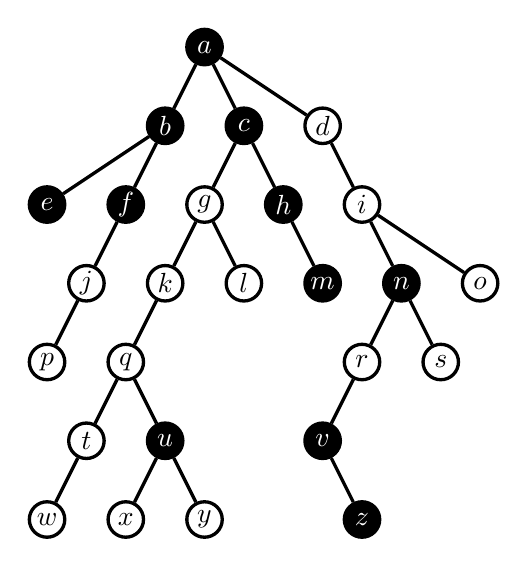
\begin{tikzpicture}[every path/.style={very thick}]
    
    \node[text=white, circle, draw, minimum size=0.45cm, inner sep=0pt, fill=black] (1) at (0,0) {$a$};

    \node[text=white, circle, draw, minimum size=0.45cm, inner sep=0pt, fill=black] (2) at (-0.5,-1) {$b$};

    \node[text=white, circle, draw, minimum size=0.45cm, inner sep=0pt, fill=black] (3) at (0.5,-1) {$c$};

    \node[circle, draw, minimum size=0.45cm, inner sep=0pt, fill=white] (4) at (1.5,-1) {$d$};

    \draw[] (1) to (2);
    \draw[] (1) to (3);
    \draw[] (1) to (4);

    \node[text=white, circle, draw, minimum size=0.45cm, inner sep=0pt, fill=black] (5) at (-2,-2) {$e$};

    \node[text=white, circle, draw, minimum size=0.45cm, inner sep=0pt, fill=black] (6) at (-1,-2) {$f$};

    \node[circle, draw, minimum size=0.45cm, inner sep=0pt, fill=white] (7) at (0,-2) {$g$};

    \node[text=white, circle, draw, minimum size=0.45cm, inner sep=0pt, fill=black] (8) at (1,-2) {$h$};

    \node[circle, draw, minimum size=0.45cm, inner sep=0pt, fill=white] (9) at (2,-2) {$i$};

    \draw[] (2) to (5);
    \draw[] (2) to (6);

    \draw[] (3) to (7);
    \draw[] (3) to (8);

    \draw[] (4) to (9);

    \node[circle, draw, minimum size=0.45cm, inner sep=0pt, fill=white] (10) at (-1.5,-3) {$j$};

    \node[circle, draw, minimum size=0.45cm, inner sep=0pt, fill=white] (11) at (-0.5,-3) {$k$};

    \node[circle, draw, minimum size=0.45cm, inner sep=0pt, fill=white] (12) at (0.5,-3) {$l$};

    \node[text=white, circle, draw, minimum size=0.45cm, inner sep=0pt, fill=black] (13) at (1.5,-3) {$m$};

    \node[text=white, circle, draw, minimum size=0.45cm, inner sep=0pt, fill=black] (14) at (2.5,-3) {$n$};

    \node[circle, draw, minimum size=0.45cm, inner sep=0pt, fill=white] (15) at (3.5,-3) {$o$};

    \draw[] (6) to (10);

    \draw[] (7) to (11);
    \draw[] (7) to (12);

    \draw[] (8) to (13);

    \draw[] (9) to (14);
    \draw[] (9) to (15);

    \node[circle, draw, minimum size=0.45cm, inner sep=0pt, fill=white] (16) at (-2,-4) {$p$};

    \node[circle, draw, minimum size=0.45cm, inner sep=0pt, fill=white] (17) at (-1,-4) {$q$};

    \node[circle, draw, minimum size=0.45cm, inner sep=0pt, fill=white] (18) at (2,-4) {$r$};

    \node[circle, draw, minimum size=0.45cm, inner sep=0pt, fill=white] (19) at (3,-4) {$s$};

    \draw[] (10) to (16);
    
    \draw[] (11) to (17);
    
    \draw[] (14) to (18);
    \draw[] (14) to (19);

    \node[circle, draw, minimum size=0.45cm, inner sep=0pt, fill=white] (20) at (-1.5,-5) {$t$};

    \node[text=white, circle, draw, minimum size=0.45cm, inner sep=0pt, fill=black] (21) at (-0.5,-5) {$u$};

    \node[text=white, circle, draw, minimum size=0.45cm, inner sep=0pt, fill=black] (22) at (1.5,-5) {$v$};

    \draw[] (17) to (20);
    \draw[] (17) to (21);

    \draw[] (18) to (22);


    \node[circle, draw, minimum size=0.45cm, inner sep=0pt, fill=white] (23) at (-2,-6) {$w$};

    \node[circle, draw, minimum size=0.45cm, inner sep=0pt, fill=white] (24) at (-1,-6) {$x$};

    \node[circle, draw, minimum size=0.45cm, inner sep=0pt, fill=white] (25) at (0,-6) {$y$};

    \node[text=white, circle, draw, minimum size=0.45cm, inner sep=0pt, fill=black] (26) at (2,-6) {$z$};

    
    \draw[] (20) to (23);

    \draw[] (21) to (24);
    \draw[] (21) to (25);

    \draw[] (22) to (26);
    
    \end{tikzpicture}
    \caption[Input tree $T$ with a heavy root]{}\label{tree_h_root}
\end{minipage}
\begin{minipage}[t]{0.49\textwidth}
    \centering
    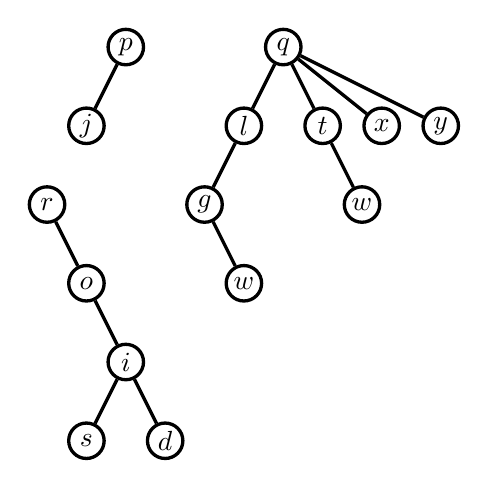
\begin{tikzpicture}[every path/.style={very thick}]
    
    \node[circle, draw, minimum size=0.45cm, inner sep=0pt, fill=white] (1) at (0,0) {$p$};

    \node[circle, draw, minimum size=0.45cm, inner sep=0pt, fill=white] (2) at (-0.5,-1) {$j$};

    \draw[] (1) to (2);

    \node[circle, draw, minimum size=0.45cm, inner sep=0pt, fill=white] (3) at (2,0) {$q$};



    \node[circle, draw, minimum size=0.45cm, inner sep=0pt, fill=white] (4) at (1.5,-1) {$l$};

    \node[circle, draw, minimum size=0.45cm, inner sep=0pt, fill=white] (5) at (2.5,-1) {$t$};

    \node[circle, draw, minimum size=0.45cm, inner sep=0pt, fill=white] (6) at (3.25,-1) {$x$};

    \node[circle, draw, minimum size=0.45cm, inner sep=0pt, fill=white] (7) at (4,-1) {$y$};

    

    \draw[] (3) to (4);
    \draw[] (3) to (5);
    \draw[] (3) to (6);
    \draw[] (3) to (7);

    \node[circle, draw, minimum size=0.45cm, inner sep=0pt, fill=white] (8) at (1,-2) {$g$};

    \node[circle, draw, minimum size=0.45cm, inner sep=0pt, fill=white] (9) at (3,-2) {$w$};

    \draw[] (4) to (8);
    \draw[] (5) to (9);

    \node[circle, draw, minimum size=0.45cm, inner sep=0pt, fill=white] (10) at (1.5,-3) {$w$};

    \draw[] (8) to (10);



    \node[circle, draw, minimum size=0.45cm, inner sep=0pt, fill=white] (11) at (-1,-2) {$r$};


    \node[circle, draw, minimum size=0.45cm, inner sep=0pt, fill=white] (12) at (-0.5,-3) {$o$};

    \draw[] (11) to (12);

    \node[circle, draw, minimum size=0.45cm, inner sep=0pt, fill=white] (13) at (0,-4) {$i$};

    \draw[] (12) to (13);

    \node[circle, draw, minimum size=0.45cm, inner sep=0pt, fill=white] (14) at (-0.5,-5) {$s$};

    \node[circle, draw, minimum size=0.45cm, inner sep=0pt, fill=white] (15) at (0.5,-5) {$d$};

    \draw[] (13) to (14);
    \draw[] (13) to (15);


    
    \end{tikzpicture}
    \caption[Input forest of decision trees for light vertices $F_C$.]{}\label{input_forest}
\end{minipage}
\begin{minipage}[t]{0.49\textwidth}
    \centering
    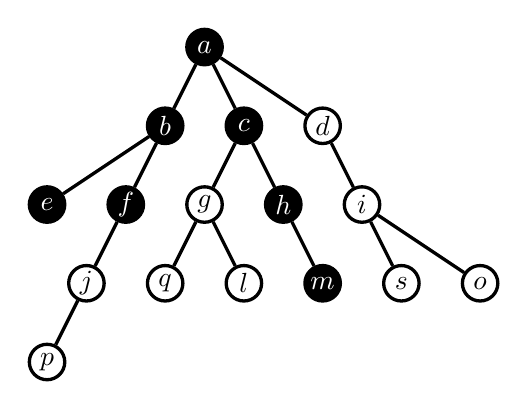
\begin{tikzpicture}[every path/.style={very thick}]
    
    \node[text=white, circle, draw, minimum size=0.45cm, inner sep=0pt, fill=black] (1) at (0,0) {$a$};

    \node[text=white, circle, draw, minimum size=0.45cm, inner sep=0pt, fill=black] (2) at (-0.5,-1) {$b$};

    \node[text=white, circle, draw, minimum size=0.45cm, inner sep=0pt, fill=black] (3) at (0.5,-1) {$c$};

    \node[circle, draw, minimum size=0.45cm, inner sep=0pt, fill=white] (4) at (1.5,-1) {$d$};

    \draw[] (1) to (2);
    \draw[] (1) to (3);
    \draw[] (1) to (4);

    \node[text=white, circle, draw, minimum size=0.45cm, inner sep=0pt, fill=black] (5) at (-2,-2) {$e$};

    \node[text=white, circle, draw, minimum size=0.45cm, inner sep=0pt, fill=black] (6) at (-1,-2) {$f$};

    \node[circle, draw, minimum size=0.45cm, inner sep=0pt, fill=white] (7) at (0,-2) {$g$};

    \node[text=white, circle, draw, minimum size=0.45cm, inner sep=0pt, fill=black] (8) at (1,-2) {$h$};

    \node[circle, draw, minimum size=0.45cm, inner sep=0pt, fill=white] (9) at (2,-2) {$i$};

    \draw[] (2) to (5);
    \draw[] (2) to (6);

    \draw[] (3) to (7);
    \draw[] (3) to (8);

    \draw[] (4) to (9);

    \node[circle, draw, minimum size=0.45cm, inner sep=0pt, fill=white] (10) at (-1.5,-3) {$j$};

    \node[circle, draw, minimum size=0.45cm, inner sep=0pt, fill=white] (11) at (-0.5,-3) {$q$};

    \node[circle, draw, minimum size=0.45cm, inner sep=0pt, fill=white] (12) at (0.5,-3) {$l$};

    \node[text=white, circle, draw, minimum size=0.45cm, inner sep=0pt, fill=black] (13) at (1.5,-3) {$m$};

    \node[circle, draw, minimum size=0.45cm, inner sep=0pt, fill=white] (14) at (2.5,-3) {$s$};

    \node[circle, draw, minimum size=0.45cm, inner sep=0pt, fill=white] (15) at (3.5,-3) {$o$};

    \draw[] (6) to (10);

    \draw[] (7) to (11);
    \draw[] (7) to (12);

    \draw[] (8) to (13);

    \draw[] (9) to (14);
    \draw[] (9) to (15);

    \node[circle, draw, minimum size=0.45cm, inner sep=0pt, fill=white] (16) at (-2,-4) {$p$};


    \draw[] (10) to (16);

    
    \end{tikzpicture}
    \caption[Medusa tree $T_M$]{}\label{medusa_tree}
\end{minipage}
\caption[Construction of the medusa tree]{Construction of the medusa tree. Figure \ref{tree_h_root} shows example input tree $T$ with a heavy root. Figure \ref{input_forest} shows example input forest of decision trees for light vertices $F_C$. Figure \ref{medusa_tree} shows the constructed medusa tree $T_M$.}\label{medusa_tree_construction_figure}
\end{figure}